\section{Method}
\label{sec:method}
\begin{figure*}[t]
    \centering
    % 请将文件名替换为你实际保存的文件名，例如 jitrl_framework.png
    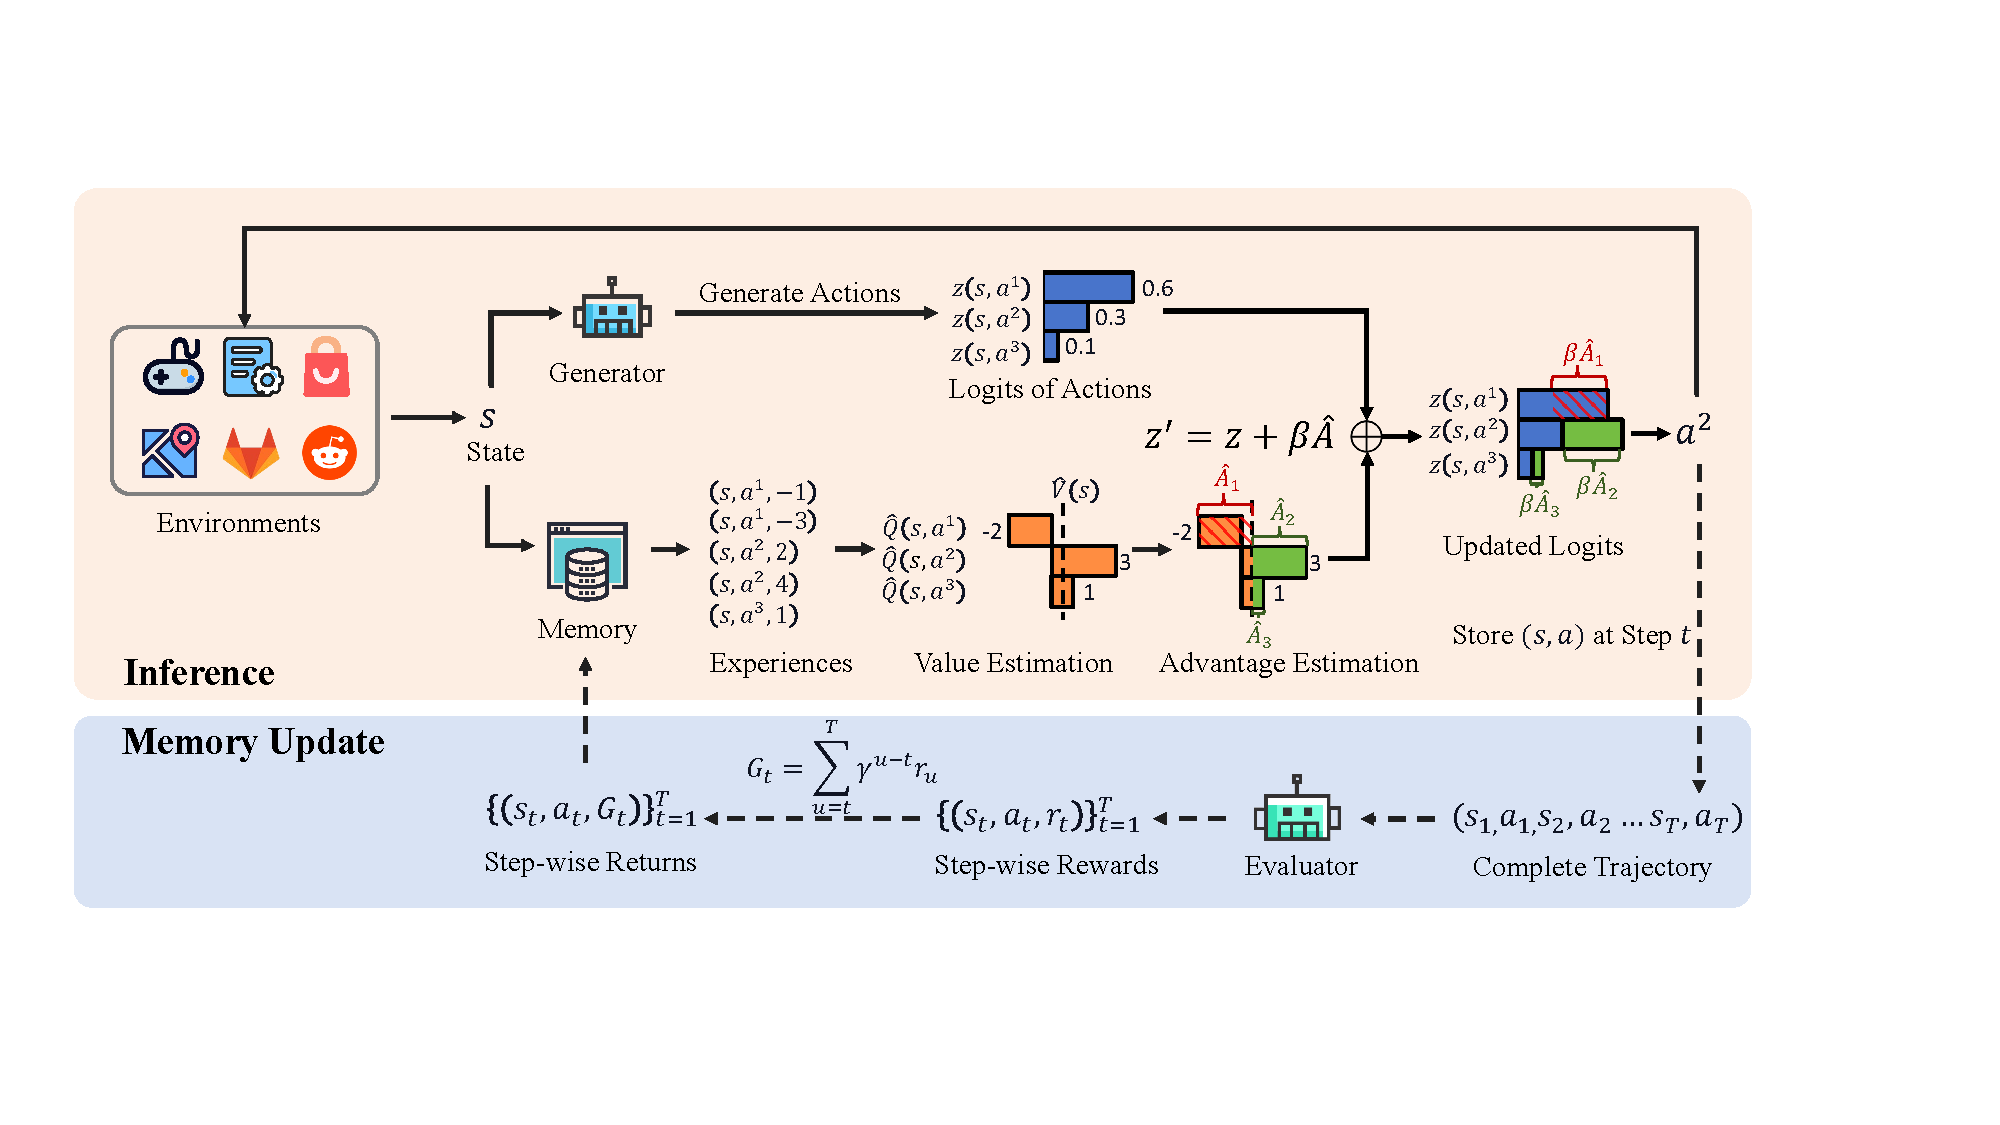
\includegraphics[width=\linewidth]{figures/framework4.pdf}
    \vspace{1mm}
    \caption{\textbf{Overview of the Just-In-Time Reinforcement Learning (JitRL) framework.} 
    The system operates in a continuous loop: 
    (1) In the \textit{Inference} (top), the agent retrieves relevant past experiences $\mathcal{N}(s)$ from the non-parametric memory $\mathcal{M}$. The base LLM's logits $z$ are then adjusted in closed-form ($z' = z + \beta \widehat A$) using the estimated advantage $A$ derived from historical returns, enabling test-time policy improvement without gradient updates. 
    (2) In the \textit{Memory Update} (bottom), completed trajectories are analyzed by an evaluator to compute discounted returns $G_t$. These new experiences are stored back into $\mathcal{M}$, allowing the agent to evolve its policy across episodes.}
    \label{fig:jitrl_framework}

\end{figure*}


To address the limitations of gradient-based RL, we present \textbf{Just-In-Time Reinforcement Learning (JitRL)} framework. Instead of updating model parameters $\theta$, JitRL functions as a test-time policy optimization method that modulates a frozen prior $\pi_{\theta}$ towards an optimal posterior $\pi^*$. As illustrated in Figure~\ref{fig:jitrl_framework}, the framework consists of three key components: (1) constructing a granular experience memory from completed trajectories, (2) estimating state and action values via retrieval during inference, and (3) dynamically updating the LLM's policy logits based on estimated advantages.  The  algorithm can be found in Appendix \ref{app:alg}.



\subsection{Memory Construction}

In the absence of a trained value network, we estimate expected returns by querying a dynamic memory $\mathcal{M} = \{(s_i, a_i, G_i)\}_{i=1}^N$. Here, $G_i$ characterizes the cumulative discounted reward observed after state $s_i$ and action $a_i$ in prior trajectories, effectively capturing the environment's empirical distribution.
%Constructing an effective memory requires bridging the gap between sparse environmental feedback (e.g., binary success/failure) and the need for dense, step-wise guidance. 

\textbf{Reflective Step-wise Rewards.} Credit assignment is challenging under long trajectories, so we use the agent's self-reflective abilities to improve credit assignment. At the end of each episode, an LLM-based \textbf{Evaluator} assesses the completed trajectory $\tau = (s_1, a_1, \dots, s_T, a_T)$ to generate step-wise rewards. This is defined by the mapping $\mathcal{E}: \tau \to \{r_t\}_{t=1}^T$, where each $r_t$ is a scalar reward quantifying the individual contribution of action $a_t$ to the overall success of the task. These rewards are then aggregated into the discounted return $G_t$ to quantify the long-term value of each action:
\begin{equation}
    G_{t}=\sum_{u=t}^{T}\gamma^{u-t}r_{u},
    \label{eq:discounted_return}
\end{equation}
where $\gamma \in [0, 1]$ balances the weight of immediate versus future rewards.

\textbf{State Construction.} Raw states (e.g., full HTML DOM trees or verbose game text) are often too noisy for effective retrieval. We abstract them into compact, structured states $s_t$ that preserve task-relevant semantics while discarding irrelevant details. Our key design principle is mapping functionally equivalent states to similar representations. Details on state construction can be found in Appendix ~\ref{app:implementation}.


% For instance, in web navigation, we normalize URLs by replacing instance-specific identifiers (e.g., product IDs) with placeholders, so that different instances of the same page type share a common representation. In text games, we extract key entities and actions into a structured format. This abstraction enables cross-instance knowledge transfer---experiences from one product page can inform decisions on another.

Ultimately, each transition is stored in the dynamic memory $\mathcal{M}$ as a compact triplet $(s_t, a_t, G_t)$, implicitly representing the empirical distribution of the environment's dynamics.



\subsection{Test-Time Value Estimation}
\label{sec:value_estimation}

Instead of relying on computationally expensive value networks, we perform on-the-fly value estimation by retrieving relevant transitions from memory. During inference, the current observation is abstracted into a structured state $s$. 
We then retrieve top-$k$ similar neighbors to form a local neighborhood $\mathcal{N}(s)$.

% \textcolor{blue}{
% We use text-based state representations. To quantify the similarity between the current state $s$ and a memory state $s_i$, we tokenize both representations and compute the \textbf{Jaccard Similarity}:
% \begin{equation}
%     J(s, s_i) = \frac{|T(s) \cap T(s_i)|}{|T(s) \cup T(s_i)|},
% \end{equation}
% where $T(\cdot)$ denotes the set of tokens derived from a state. 
% }

We formulate the \textbf{ state value} estimation $\widehat V(s)$ for state $s$ as an expectation of the returns across this neighborhood:
\begin{equation}
       \widehat V(s)\coloneqq \frac{1}{|\mathcal{N}(s)|} \sum_{i \in \mathcal{N}(s)} G_i. %\xrightarrow{p} \mathbb{E}_{\tau \sim \mathcal{N}(s)}[G].
\end{equation}
Similarly, to evaluate a specific candidate action $a$, we condition the \textbf{action value} $\widehat Q(s,a)$ on the state-action pair $(s,a)$ over the relevant subset $\mathcal{N}(s, a) = \{(s_i, a_i, G_i) \in \mathcal{N}(s) : a_i = a\}$: We distinguish between two cases:

\begin{enumerate}[leftmargin=*, nosep, label=\textbf{\arabic*.}]
\item \textbf{Known Actions:} If historical evidence exists (i.e., $|\mathcal{N}(s, a)| > 0$), we estimate the action value by averaging the returns within the subset:
\begin{equation}
\begin{aligned}
\widehat Q(s,a)\coloneqq \frac{1}{|\mathcal{N}(s,a)|} \sum_{j \in \mathcal{N}(s,a)} G_j.  %\xrightarrow{p} \mathbb{E}_{\tau \sim \mathcal{N}(s,a)}[G].
\end{aligned}
\label{eq:value_est}
\end{equation}

\item \textbf{Unseen Actions:} For actions lacking historical data (i.e., $|\mathcal{N}(s, a)| = 0$), we encourage exploration by adopting an optimism under uncertainty principle. With probability $\lambda$, we assign an optimistic value:
\begin{equation}
\widehat Q(s,a) \coloneqq \widehat  V(s) + \frac{\alpha}{|\mathcal{N}(s)|}.
\label{eq:exploration}
\end{equation}
\end{enumerate}
The bonus $\alpha / |\mathcal{N}(s)|$ reflects epistemic uncertainty: sparse memory coverage (small $|\mathcal{N}(s)|$) implies unreliable estimates, warranting exploration. As experiences accumulate, the bonus diminishes, naturally shifting toward exploitation. With probability $1-\lambda$, we assign $Q(s,a) = 0$ to prevent over-exploration.

The \textbf{test-time advantage} is then derived by centering the action value against the state baseline:
\begin{equation}
    \widehat A(s,a) = \widehat Q(s,a) - \widehat V(s).
    \label{eq:test_time_advantage}
\end{equation}
This allows us to identify actions that outperform the local average purely through inference-time retrieval, serving as a proxy for the advantage function $A^{\pi}(s,a)$.




\subsection{Policy Update}
\label{sec:policy_update}



Given these value estimates, we formally derive the policy update as a constrained optimization problem. We seek an optimal policy:
\begin{equation}
    \pi^* = \arg \max_{\pi'} \left( \mathbb{E}_{a \sim \pi'} [ A(s,a)] - \frac{1}{\beta} D_{KL}(\pi' || \pi_{\theta}) \right),
    \label{eq:optimization_objective}
\end{equation}
where $\beta$ is the temperature hyperparameter. Eq. ~\eqref{eq:optimization_objective} maximizes the expected advantage while minimizing the KL-divergence from the frozen reference policy $\pi_{\theta}$ to preserve linguistic coherence. The closed-form solution to this optimization objective is:
\begin{equation}
    \pi^*(a|s) \propto \pi_{\theta}(a|s) \exp\left( \beta A(s,a) \right)
    \label{eq:optimal_policy}
\end{equation}
where $\beta$ is the temperature parameter that controls the strength of the constraint. 

To implement this optimal policy without gradient updates, we map Eq.~\eqref{eq:optimal_policy} directly to the logit space. Let $z(s,a)$ be the logits of the base LLM such that $\pi_{\theta}(a|s) = \text{Softmax}(z(s,a))$. Taking the logarithm of Eq.~\eqref{eq:optimal_policy} yields an additive update rule:
\begin{equation}
    z'(s,a) = z(s,a) + \beta \cdot  \widehat A (s,a)
    \label{eq:logit_update}
\end{equation}
By applying the Softmax function to the updated logits $z'(s,a)$, we recover the optimal policy distribution $\pi^*$. 






\subsection{Theoretical Analysis}
\label{subsec:theoretical_analysis}

We provide theoretical justification for JitRL through three progressive steps. First, we prove our logit update is the exact closed-form solution for KL-constrained optimization (Theorem 4.1). Next, we demonstrate that our value estimates converge to the true values (Theorem 4.2), ensuring the overall policy update consistently converges to the optimal policy (Theorem 4.3). Detailed statements and proofs can be found in Appendix~\ref{app:derivation}, ~\ref{app:consistency}, and ~\ref{app:cons_policy}.

\paragraph{Optimality of Logit Update.}
We formulate the inference-time adjustment as a constrained optimization problem. Our goal is to find a policy $\pi'$ that effectively utilizes the retrieved advantage information while preserving the linguistic capabilities of the pre-trained model.

\begin{theorem}[Optimality of Policy Update]
\label{thm:closed_form}
Let $\pi_{\theta}$ be the reference policy with logits $z(s,a)$. Consider the problem of finding the optimal policy $\pi^*$ that maximizes the expected advantage subject to a KL-divergence penalty:
\begin{equation}
    \pi^* = \arg \max_{\pi'} \left( \mathbb{E}_{a \sim \pi'} [\widehat A(s,a)] - \frac{1}{\beta} D_{KL}(\pi' || \pi_{\theta}) \right)
    \label{eq:optimization_objective2}
\end{equation}
where $\beta$ is a temperature hyperparameter. The solution to this optimization problem is given by the additive logit update:
\begin{equation}
    z'(s,a) = z(s,a) + \beta \cdot \widehat A(s,a)
    \label{eq:logit_update_rule}
\end{equation}
where $z'(s,a)$ denotes the logits of the optimal policy $\pi^*$.
\end{theorem}

\paragraph{Consistency of Value and Advantage Estimates.}
Next, we show that the estimators $\widehat{V}_t$, $\widehat{Q}_t$, and $\widehat{A}_t$ converge in probability to their true counterparts $V^{\pi_t}$, $Q^{\pi_t}$, and $A^{\pi_t}$, even under the non-stationary policy setting $(\pi_t)_{t \ge 1}$.

\begin{theorem}[Consistency of $\widehat V_t$, $\widehat Q_t$, and $\widehat A_t$]\label{thm:tracking_QV}
Under the assumptions given in Appendix \ref{app:consistency}, for any fixed query state $s$ and action $a$ at time
$t$, as $t\to\infty$,
\begin{align*}
\widehat V_t(s) & \xrightarrow{p} V^{\pi_t}(s),\\
\widehat Q_t(s,a) & \xrightarrow{p} Q^{\pi_t}(s,a), \\
\widehat A_t(s,a) & \xrightarrow{p} A^{\pi_t}(s,a).
\end{align*}
\end{theorem}

\paragraph{Consistency of Policy Update.}
Finally, combining the previous two theorems, we conclude that our policy update converges to the KL-regularized optimal policy induced by the true advantages $A^{\pi_t}$:

\begin{theorem}[Consistency of Policy Update]
\label{cor:policy_consistency}
Fix a state $s$, and define
\begin{align*}
\pi_t^*(a\mid s)\propto \pi_\theta(a\mid s)\exp\!\big(\beta A^{\pi_t}(s,a)\big),\\
\widehat\pi_t(a\mid s)\propto \pi_\theta(a\mid s)\exp\!\big(\beta \widehat A_t(s,a)\big).
\end{align*}
Under the assumptions of Theorem~\ref{thm:tracking_QV},
as $t\to\infty$,
\[
\widehat\pi_t(\cdot\mid s) \xrightarrow[]{p} \pi_t^*(\cdot\mid s),
\]
for any finite candidate action set (or more generally, under uniform convergence of $\widehat A_t(s,\cdot)$ on the candidate set).
\end{theorem}






% \paragraph{Consistency of Value Estimation.}
% The validity of the update relies on the accuracy of the estimated action values. We examine whether our retrieval-based estimator converges to the true action value.

% \begin{theorem}[Consistency of Value Estimation]
% \label{thm:consistency}
% Let $\hat{Q}(s,a)$ be the value estimated using $k$-nearest neighbors from memory $\mathcal{M}$ of size $N$. Assume: (i) the true action-value function $Q^{\pi}(s,a)$ is Lipschitz continuous with respect to the embedding space, and (ii) the memory samples are i.i.d. drawn from the state-action distribution. If $N \to \infty$, $k \to \infty$, and $k/N \to 0$, then the estimator is consistent:
% \begin{equation}
%     \hat{Q}(s,a) \xrightarrow{p} Q^{\pi}(s,a).
% \end{equation}
% \end{theorem}

% See Appendix~\ref{app:proof_consistency} for the full proof via bias-variance decomposition.

% Combining Theorem~\ref{thm:closed_form} and Theorem~\ref{thm:consistency}, we conclude that as the memory scales, JitRL asymptotically approximates the theoretically optimal policy update step.